\chapter{Results and Discussion}

BIG REWORK

Outcomes of each trajectory case are presented in the context of guidance law performance. Consideration of the methodology is used to explain some of the observed behaviours, and deficiencies are noted for improvement.

\section{Baseline Case Runs}
This section covers the baseline trajectory cases outlines in Tables \ref{tab:trajectory_cases} and \ref{tab:trajectory_case_params}.

Table \ref{tab:outputs_1_summary} summarizes the outcomes of each case. Discussion proceeds.
\begin{table}[H]
    \centering
    \begin{tabular}{L{3cm}L{3cm}L{2.5cm}L{2.5cm}R{3cm}}
        \toprule
        \textbf{Case} & Convergence Tolerance & Time of Flight (d) & Number of Revolutions & $\Delta v$ Expenditure (m/s) \\
        \midrule
        GEO Disposal  & 0.005                 & 62.44              & 62                    & 13.1                         \\
        Plane Change  & 0.005                 & 1020               & 1944                  & 13570.3                      \\
        ``Benchmark'' & 0.005                 & 610                & 858                   & 6673.2                       \\
        Polar GSO     & 0.03                  & 490                & 494                   & 9686.7                       \\
        \bottomrule
    \end{tabular}
    \caption{Summary of outcomes for each case.}
    \label{tab:outputs_1_summary}
\end{table}

Overall, it is evident that despite being convergent, the guidance law is extremely slow in bringing the spacecraft to the target orbit.

The low thrust produced by the sail is not the key issue; rather, it is the lack of availability of thrust in a given direction. For example, a continuous thrust plane change maneuver involves continuously changing the direction of applied thrust. The direction desired by the first stage of the guidance law is not always available, and the solar sail often ends up being feathered (this effect has not yet been quantified; pending measurement of time spent in degraded/feathered operational mode).

Part of the issue with the long time of flight is the convergence tolerance (measured as the sum of the squares of the error in each element, weighed by $W_{\moe}$; this will be changed to the value of $Q$ in the future). The guidance law can reach an error of about 0.05 reasonably quickly, but spends a substantial amount of time finely correcting its trajectory at the end, resulting in very slow convergence to the final threshold.

For initial orbits very close to the target orbit (e.g. GEO disposal case), the guidance law struggles with closing the gap, and often results in extremely long missions. Altering guidance weights helps with this somewhat (see the guidance weights of the GEO disposal case, for example), but it is currently unknown whether there are also numerical artifacts to consider.

More insights are evident through inspection of the plots of the trajectory and orbital elements. Discussion on these is presented in the next section.

\section{Global Optimization Runs}
Global weight optimization was performed for the latter two baseline cases. The optimized guidance law tunings are compared against their unoptimized counterparts in Table \ref{tab:outputs_2_summary}.

\begin{table}[H]
    \centering
    \begin{tabular}{L{5cm}L{2.5cm}L{2.5cm}L{3cm}}
        \toprule
        \textbf{Case}                                     & Time of Flight (d) & Number of Revolutions & $\Delta v$ Expenditure (m/s) \\
        \midrule
        ``Benchmark'', baseline                           & 610                & 858                   & 6673.2                       \\
        \rowcolor{green!20!white}``Benchmark'', optimized & 388                & 622                   & 6193.0                       \\
        Polar GSO, baseline                               & 490                & 494                   & 9686.7                       \\
        \rowcolor{green!20!white} Polar GSO, optimized    & 375                & 323                   & 8352.0                       \\
        \bottomrule
    \end{tabular}
    \caption{Comparison of optimized cases against their baselines.}
    \label{tab:outputs_2_summary}
\end{table}

The two cases still use their original convergence tolerances in the optimized tunings.

Plots of the trajectories and orbital elements are shown in Sections \ref{sec:bench_case_plot} and \ref{sec:gso_case_plot}.

\subsection{Benchmark Case}
\label{sec:bench_case_plot}
Baseline $W_{\moe}$: $\{1, 1, 1, 1, 1\}$
\begin{figure}[H]
    \centering
    \begin{subfigure}[t]{0.49\textwidth}
        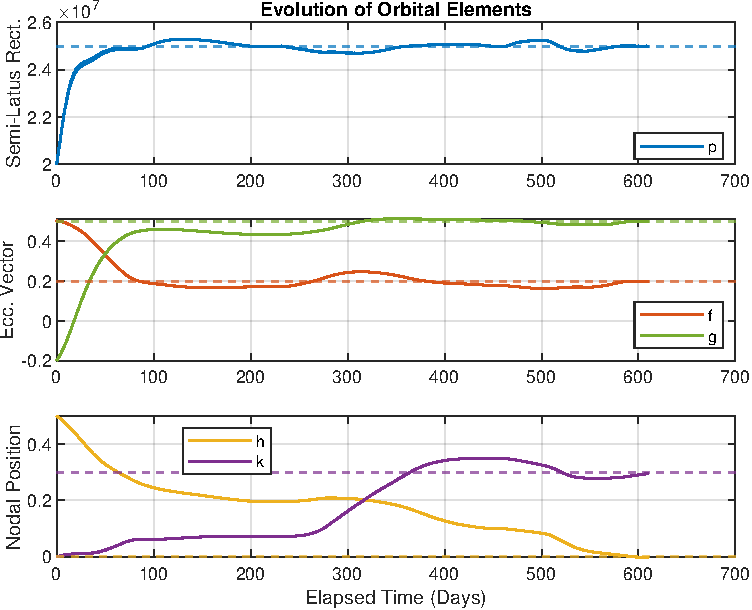
\includegraphics[width=\textwidth]{figures/benchmark_transfer/orbital_elements.pdf}
        \caption{Evolution of orbit elements in time.}
        \label{fig:results_benchmark_a}
    \end{subfigure}
    \begin{subfigure}[t]{0.49\textwidth}
        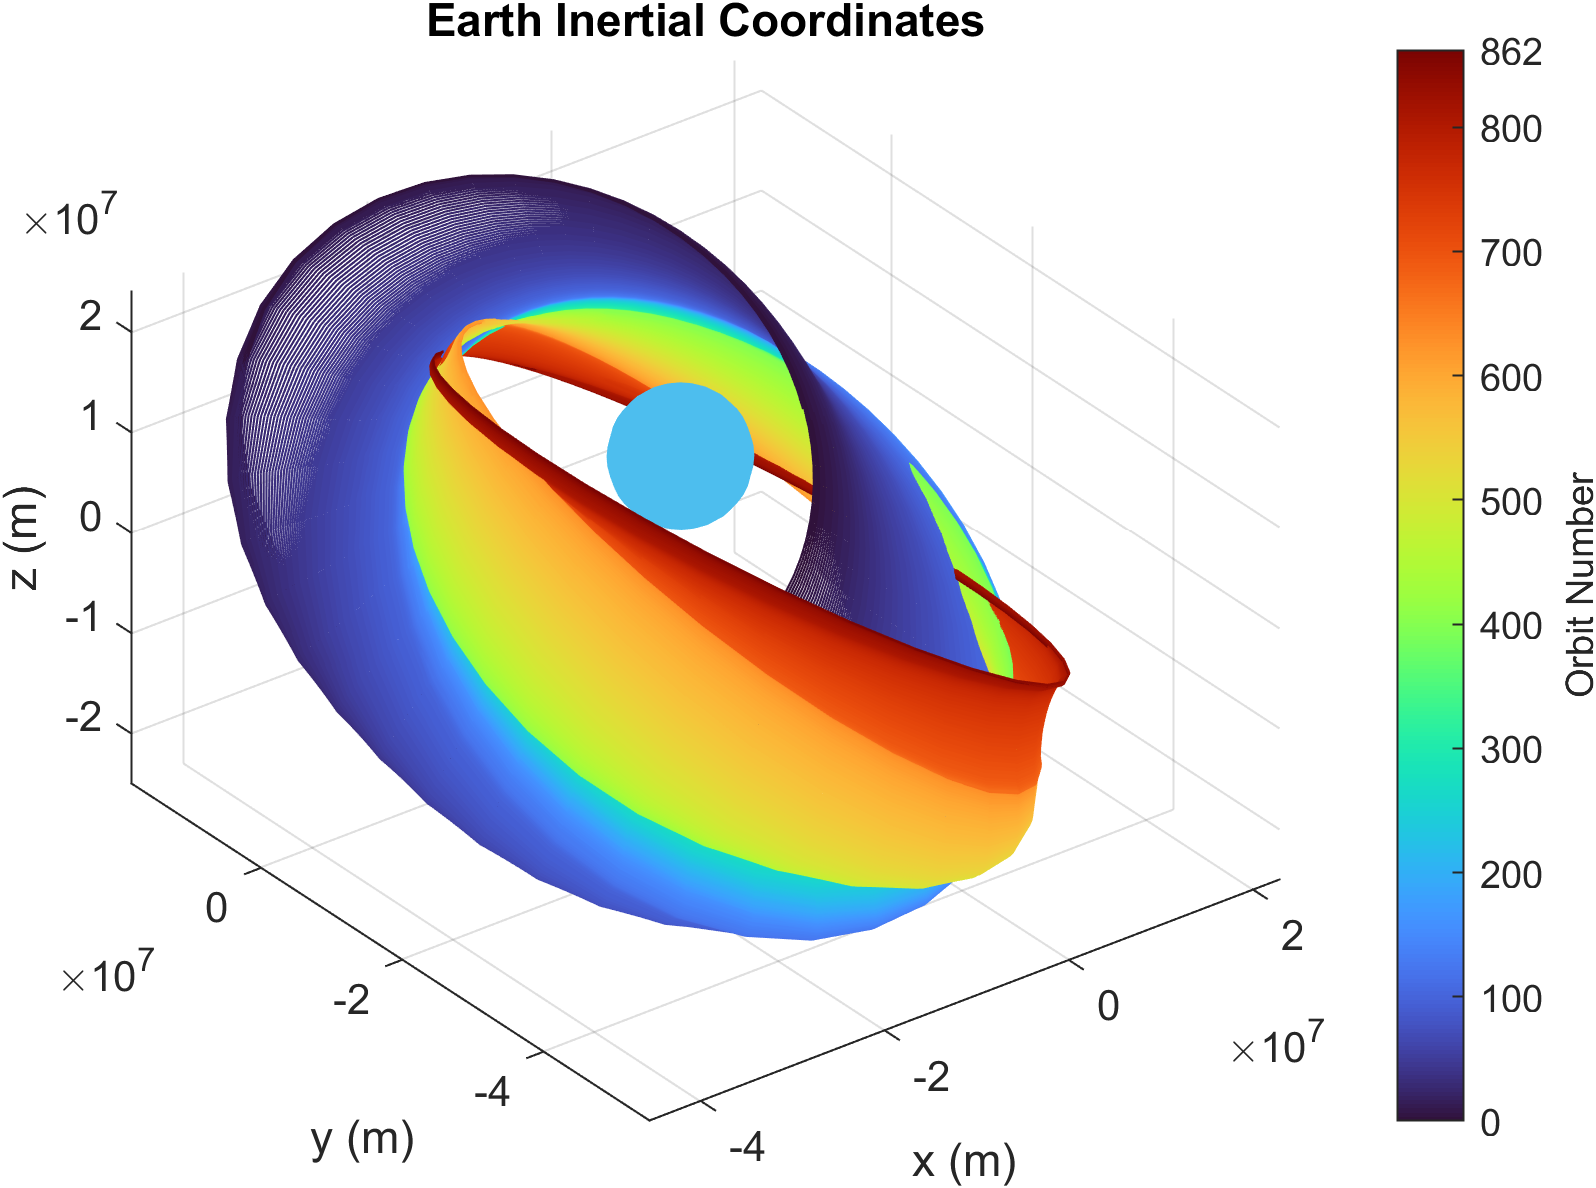
\includegraphics[width=\textwidth]{figures/benchmark_transfer/trajectory_plot.png}
        \caption{Trajectory plot.}
        \label{fig:results_benchmark_b}
    \end{subfigure}
    \caption{Benchmark transfer case, baseline.}
    \label{fig:results_benchmark}
\end{figure}

Optimal $W_{\moe}$: $\{1.774, 0.5149, 0.3327, 9.925, 0.5317\}$

\begin{figure}[H]
    \centering
    \begin{subfigure}[t]{0.49\textwidth}
        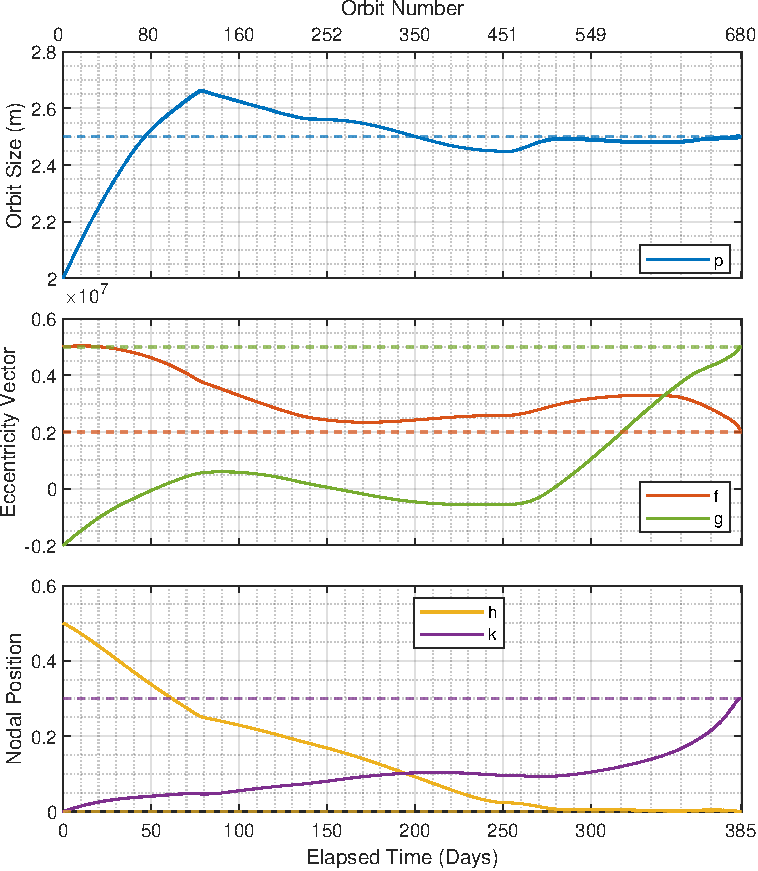
\includegraphics[width=\textwidth]{figures/benchmark_optim/orbital_elements.pdf}
        \caption{Evolution of orbit elements in time.}
        \label{fig:results_benchmark_optim_a}
    \end{subfigure}
    \begin{subfigure}[t]{0.49\textwidth}
        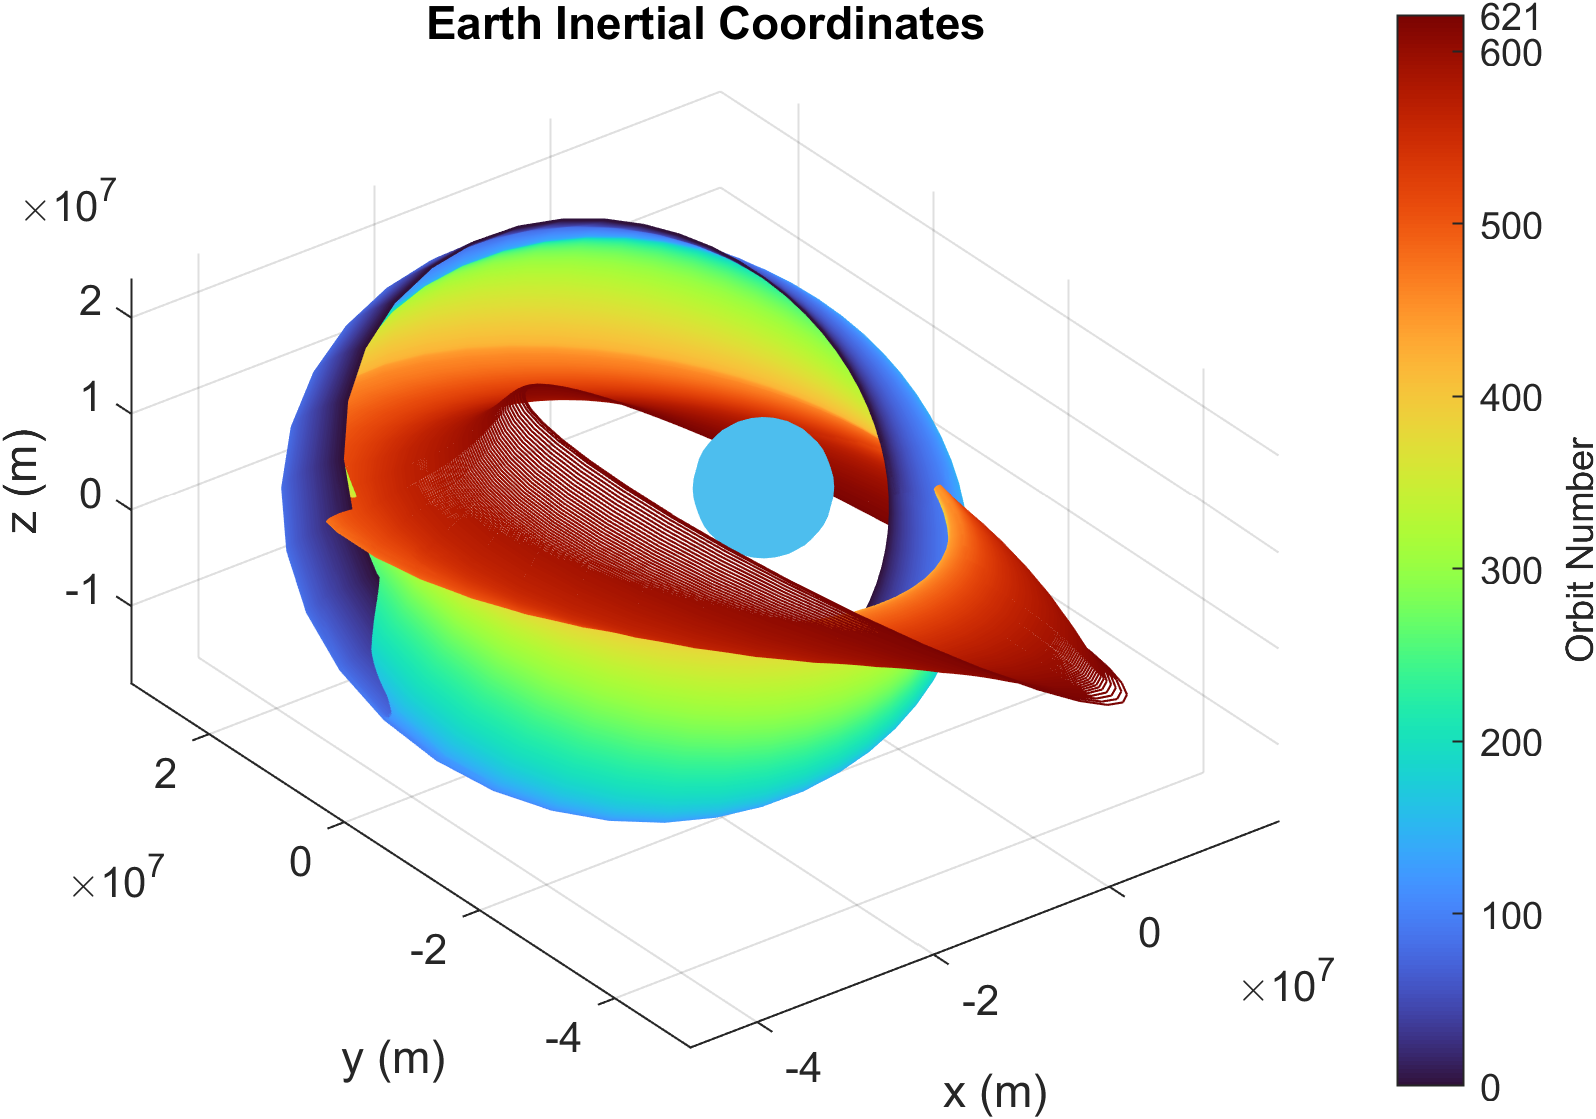
\includegraphics[width=\textwidth]{figures/benchmark_optim/trajectory_plot.png}
        \caption{Trajectory plot.}
        \label{fig:results_benchmark_optim_b}
    \end{subfigure}
    \caption{Benchmark transfer case, optimal tuning.}
    \label{fig:results_benchmark_optim}
\end{figure}

\newpage
\subsection{Polar GSO Case}
\label{sec:gso_case_plot}
Baseline $W_{\moe}$: $\{1, 1, 1, 1, 1\}$
\begin{figure}[H]
    \centering
    \begin{subfigure}[t]{0.49\textwidth}
        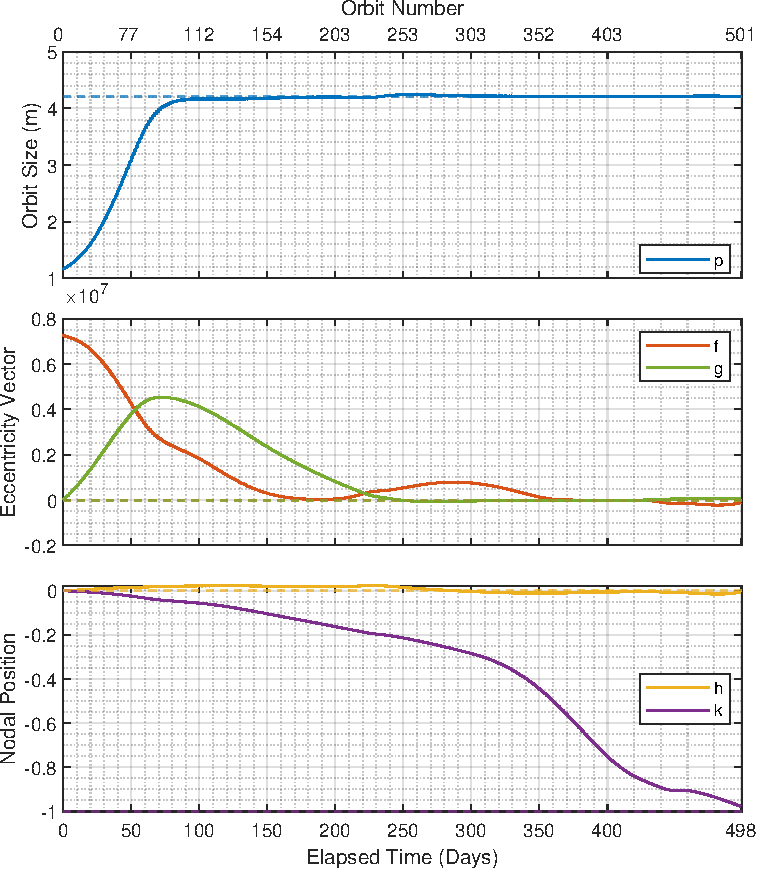
\includegraphics[width=\textwidth]{figures/oguri_G/orbital_elements.pdf}
        \caption{Evolution of orbit elements in time.}
        \label{fig:oguri_base_a}
    \end{subfigure}
    \begin{subfigure}[t]{0.49\textwidth}
        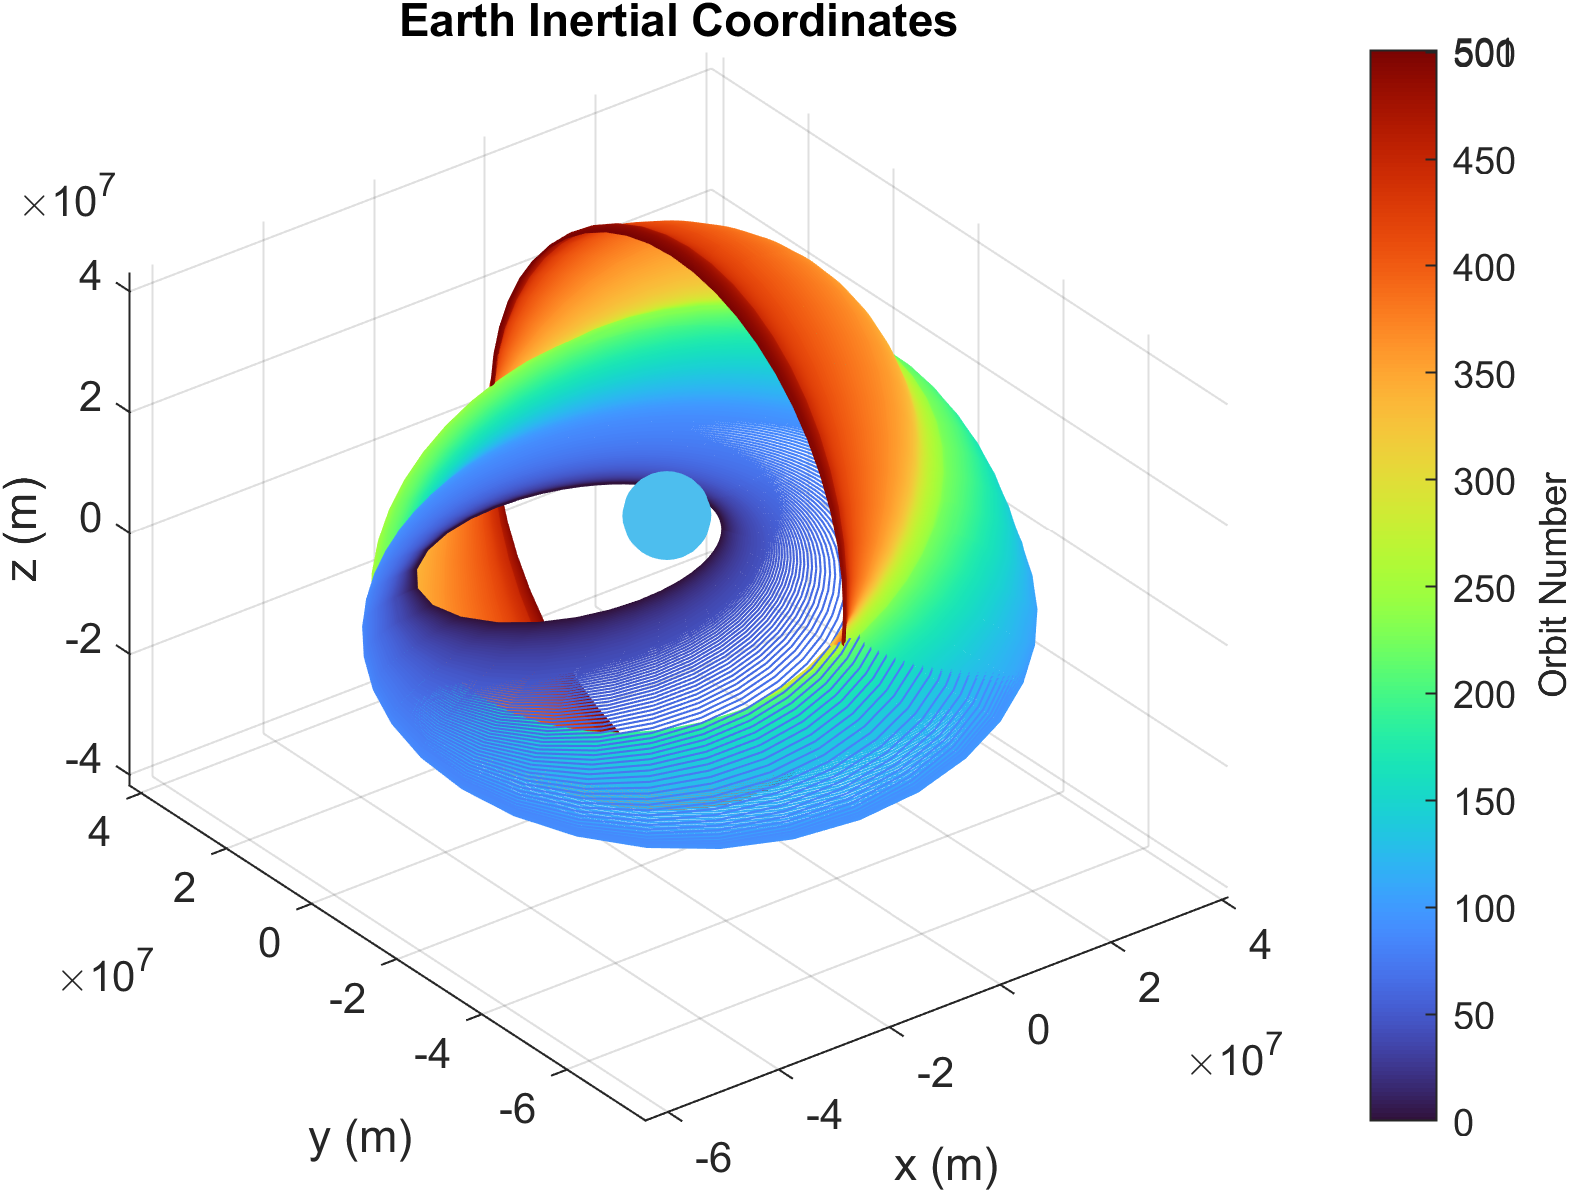
\includegraphics[width=\textwidth]{figures/oguri_G/trajectory_plot.png}
        \caption{Trajectory plot.}
        \label{fig:oguri_base_b}
    \end{subfigure}
    \caption{GTO to polar transfer, baseline.}
    \label{fig:oguri_base}
\end{figure}

Optimal $W_{\moe}$: $\{8.959, 2.132, 1.722, 3.559, 9.789\}$

\begin{figure}[H]
    \centering
    \begin{subfigure}[t]{0.49\textwidth}
        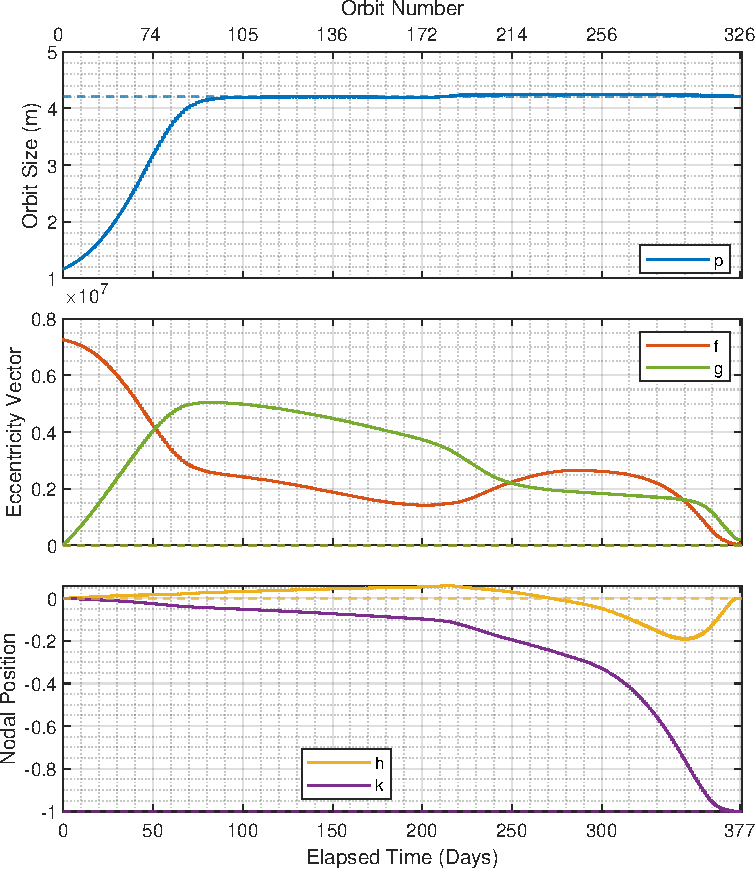
\includegraphics[width=\textwidth]{figures/oguri_optim/orbital_elements.pdf}
        \caption{Evolution of orbit elements in time.}
        \label{fig:oguri_optim_a}
    \end{subfigure}
    \begin{subfigure}[t]{0.49\textwidth}
        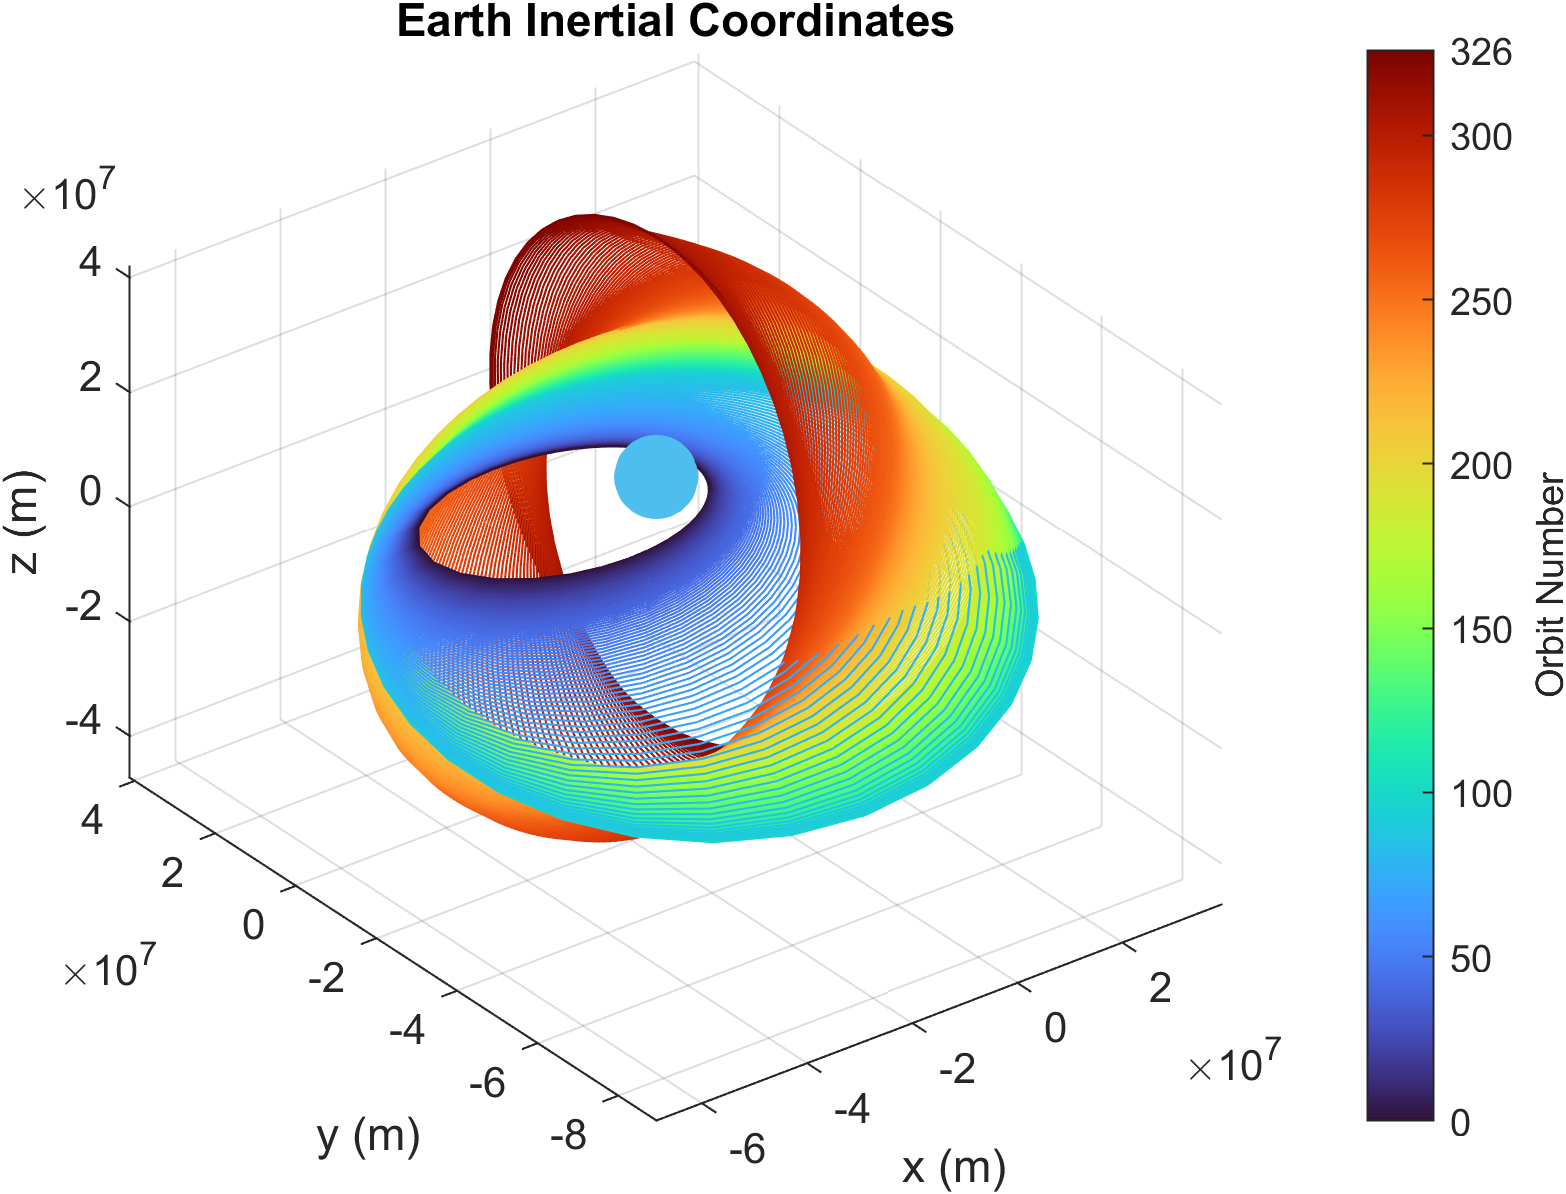
\includegraphics[width=\textwidth]{figures/oguri_optim/trajectory_plot.png}
        \caption{Trajectory plot.}
        \label{fig:oguri_optim_b}
    \end{subfigure}
    \caption{GTO to polar transfer, optimal tuning.}
    \label{fig:oguri_optim}
\end{figure}

{
\Large
Note: animated versions of the trajectory plots can be found on \href{https://github.com/itchono/SLyGA/wiki/Case-Outputs}{this webpage}.
}